In diesem Kapitel werden die spezifischen Erkenntnisse zur Regressionsaufgabe dargestellt und analysiert. Zunächst erfolgt die Einführung der 
beiden Netzarchitekturen – Deep Cascade und Direct Cascade –, um darauf aufbauend einen Vergleich zwischen den Varianten Cascade mit 
Transferlernen (TF), Cascade ohne TF sowie der jeweiligen Komplettversionen der Netzwerke unter Bedingungen mit vielen bzw. wenigen Target-Daten 
vorzunehmen. Dabei zeigen sich deutliche Unterschiede zwischen Deep und Direct Cascade, wobei insgesamt eine prinzipielle Funktionsfähigkeit 
beider Ansätze bestätigt werden kann. Abschließend werden Early-Stopping-Metriken angewendet und deren Ergebnisse diskutiert.

Die beiden Regressionsnetzwerke werden im Folgenden im Detail vorgestellt. Beide Modelle erhalten als Eingabe tabellarische Daten mit drei 
Merkmalen (Spalten), deren genaue Beschreibung bereits im Kapitel 2 erfolgte. Für das Training kommt in beiden Fällen der 
Adam-Optimizer in Kombination mit der Mean-Squared-Error-Verlustfunktion zum Einsatz. Der Ausgabeschicht entspricht einem typischen 
Regressions-Setup: ein einzelner linearer Layer mit einer Neuroneneinheit und linearer Aktivierungsfunktion.

\begin{figure}[htpb]
    \centering
    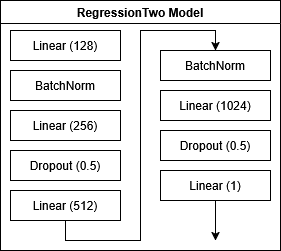
\includegraphics[height=6cm]{../../Graphiken/regressiontwo_2.png}
    \caption{\label{fig:regr2} 
    \small{In dieser Abbildung ist die Architektur des Regr2-Netzwerks im Detail dargestellt. Die Anordnung der Schichten erfolgt von oben nach 
    unten entlang der angegebenen Pfeilrichtung. Bei den Linear-Schichten ist die jeweilige Anzahl der enthaltenen Neuronen angegeben; bei den 
    Dropout-Schichten gibt der Wert den Prozentsatz der Neuronen an, die während des Trainings zufällig deaktiviert werden.}}
\end{figure}

In Abbildung \ref{fig:regr2} ist die vollständige Architektur des Regr2-Netzwerks dargestellt. Es handelt sich dabei um ein Deep-Cascade-Netzwerk, 
bei dem die Schichten schrittweise – also Layer für Layer – trainiert werden. Die Zahl hinter den Linear-Schichten gibt jeweils die Anzahl der 
enthaltenen Neuronen an, während die Angabe hinter den Dropout-Schichten den Anteil (bezogen auf den Wert 1) der während des Trainings pro 
Epoche deaktivierten Neuronen beschreibt.

Das sogenannte 1Lay-Netzwerk stellt das Direct-Cascade-Regressionsmodell dar. Es besteht aus einem einzigen Hidden Layer in Form einer 
Linear-Schicht mit 128 Neuronen und verwendet die ReLU-Aktivierungsfunktion. Dieses Netzwerk wird iterativ eingesetzt, wobei zwischen den 
einzelnen Trainingsdurchläufen Wissen in Form eines Augmented Vectors übertragen wird. Dieser Vektor entsteht, indem die Vorhersage des 
jeweils vorherigen Netzwerks als zusätzliche Spalte zur ursprünglichen Input-Tabelle hinzugefügt wird. Die erweiterte Eingabematrix dient 
anschließend als Input für das nachfolgende Netzwerk.
